\chapter{楽譜IME}
\label{chap:ime}

本章では楽譜入力を支援する楽譜IMEを提案する。

\newpage

\section{ABCの問題点}
前章までに提案したハイパー楽譜システムでは、Wiki上での楽譜入力を実現するために、テキストベースでの楽譜記述を可能とするABCを利用している。
ABCはシンプルだが、
\begin{enumerate}
    \item 記法を覚える必要がある
    \item WYSIWYGでない
\end{enumerate}という問題点が存在する。
このうち2.はハイパー楽譜システムのリアルタイムな楽譜描画によって解決されている。
1.の解決には、文字変換を行う日本語入力システム(IME)的アプローチが有効であると考えられる。
本章では楽譜IMEを提案し、既存システムと比較しても遜色ない快適な楽譜入力を実現する。

\section{楽譜IME}
楽譜IMEは楽譜辞書を利用した変換機能によりABC特有の記法や様々な楽譜の入力をサポートする。
これは前章で実装したハイパー楽譜システムの一部として利用できる。
本節では主な機能や利用フローを解説する。

\subsection{利用できる機能}
\begin{enumerate}
    \item ABC入力支援機能
    \begin{itemize}
        \item ドレミ変換機能\\
        「ドレミ」のようなカタカナ音名をABCに変換する。ABCで利用される英語音名に慣れていなくても楽譜入力が可能になる。
        \item 記号変換機能\\
        「 $\sharp\;\;\flat\;\;\natural$ 」といった臨時記号をABCに変換する。ABCでは $\sharp\;\;\flat\;\;\natural$ をそれぞれ \verb|^ _ =| と表記するが、見慣れた記号をそのまま利用できることで、感覚的な入力が可能になる。
        \item オクターブ変更機能\\
        上下キーによって音符のオクターブを変更する。ABCではオクターブ上を\texttt{'}、下を\texttt{,}と表記するが、矢印キーを利用することで感覚的な入力が可能になる。
        \item MIDIデバイス入力機能\\
        MIDIキーボードといったデバイスから直接音符を入力する。
        既存の楽譜作成ソフトでは一般的な機能であり、鍵盤を利用することで感覚的な入力が可能になる。
    \end{itemize}
    \item 楽譜入力支援機能\\
    楽譜辞書を利用した変換機能によって楽譜の入力を支援する。
    例えばCメジャーの和音(ドミソ)を入力したいときは、\texttt{C}と入力するだけで変換が可能になる。
    ABCでは和音を入力するとき\texttt{[ceg]}のように構成音を全て記述する必要があるが、よく使う三和音などはその名前から変換できるようにすることで、楽譜入力の手間を軽減する。
\end{enumerate}

\subsection{利用フロー}
\begin{enumerate}
    \item 楽譜IMEの起動\\
    コードブロック内で\mbox{Esc}キーを押すと楽譜IMEが起動する(図\ref{ime})。
    \item 文字入力\\
    文字入力すると、入力中のABCテキストからリアルタイムに楽譜がプレビューされる(図\ref{candidate})。
    変換候補も同様に楽譜として表示される。
    ここでは\texttt{"C"}という入力に対して、Cメジャー、Cマイナーの和音が候補として提示されている。
    \item 変換候補の選択\\
    文字入力中にSpaceキーを押すと変換候補を選択できる(図\ref{select})。
    \item 変換候補の入力\\
    変換候補を選択した状態でEnterキーを押すと、その楽譜を入力できる(図\ref{input})。
\end{enumerate}

\begin{figure}[H]
    \centering
    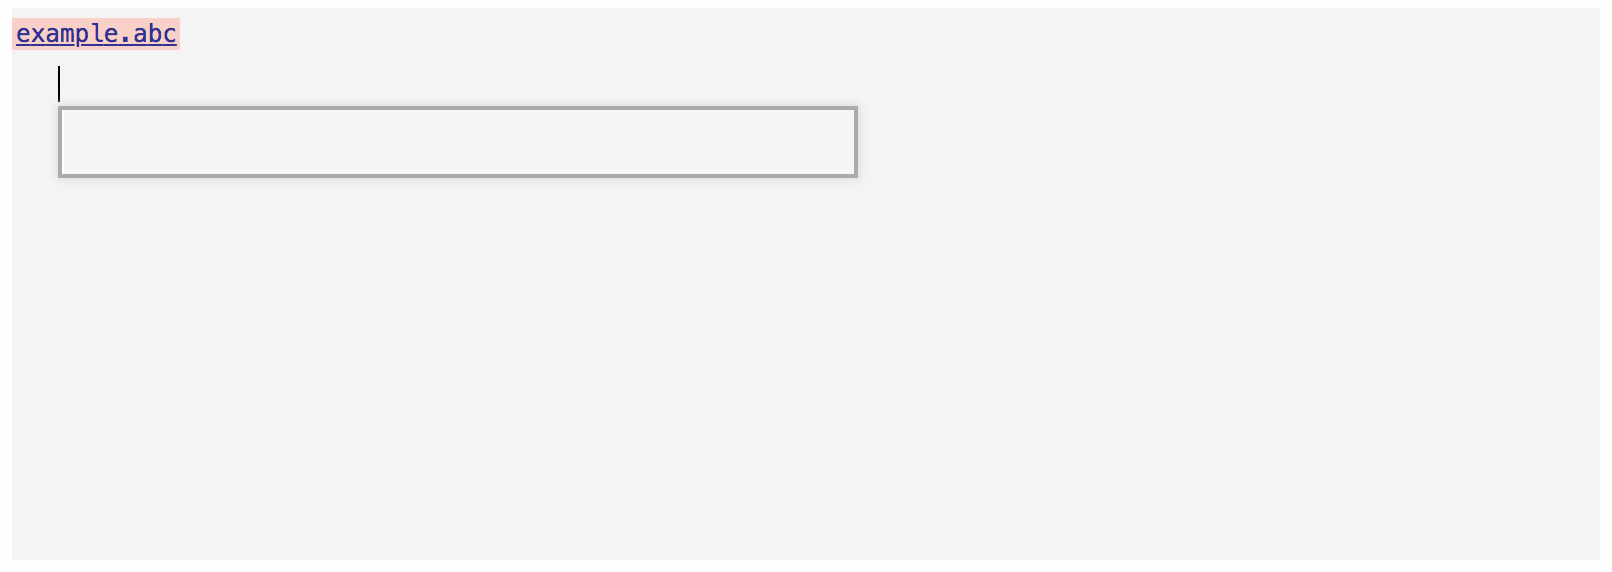
\includegraphics[width=13cm]{images/ime.png}
    \caption{楽譜IME初期画面}
    \label{ime}
\end{figure}

\begin{figure}[H]
    \centering
    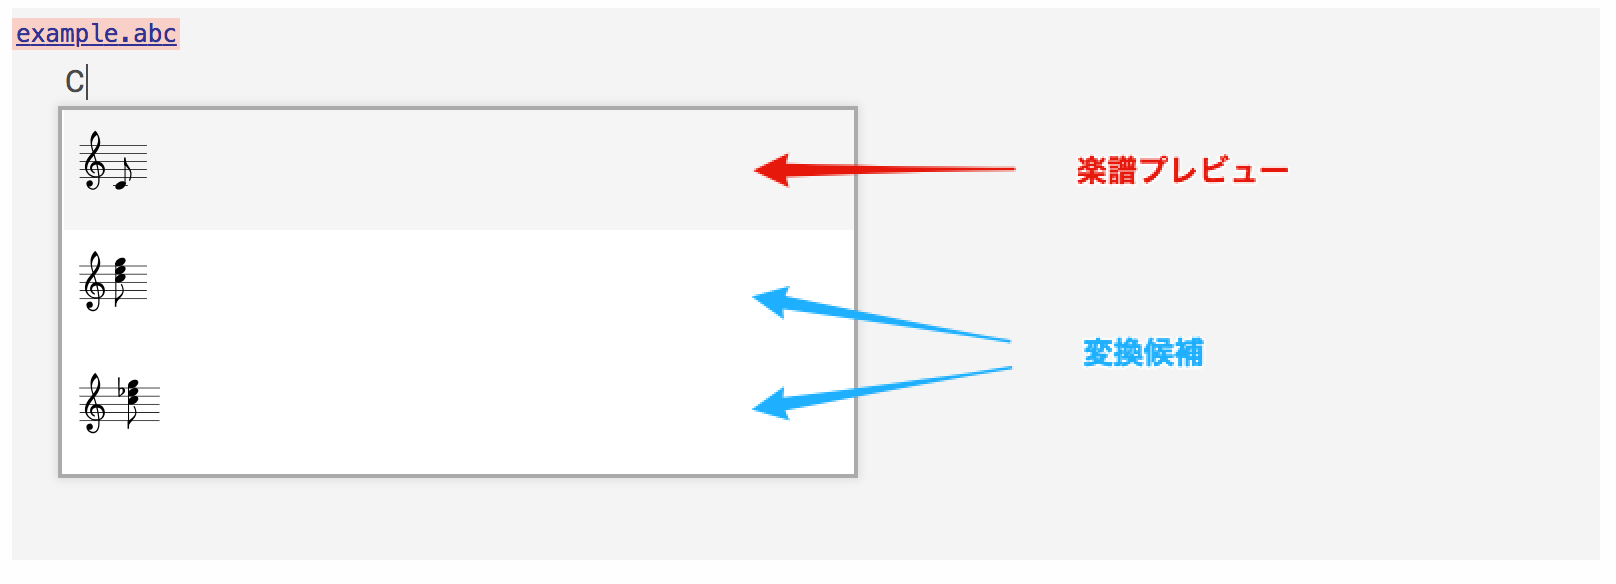
\includegraphics[width=13cm]{images/imecandidate.png}
    \caption{文字入力中の画面}
    \label{candidate}
\end{figure}

\begin{figure}[H]
    \centering
    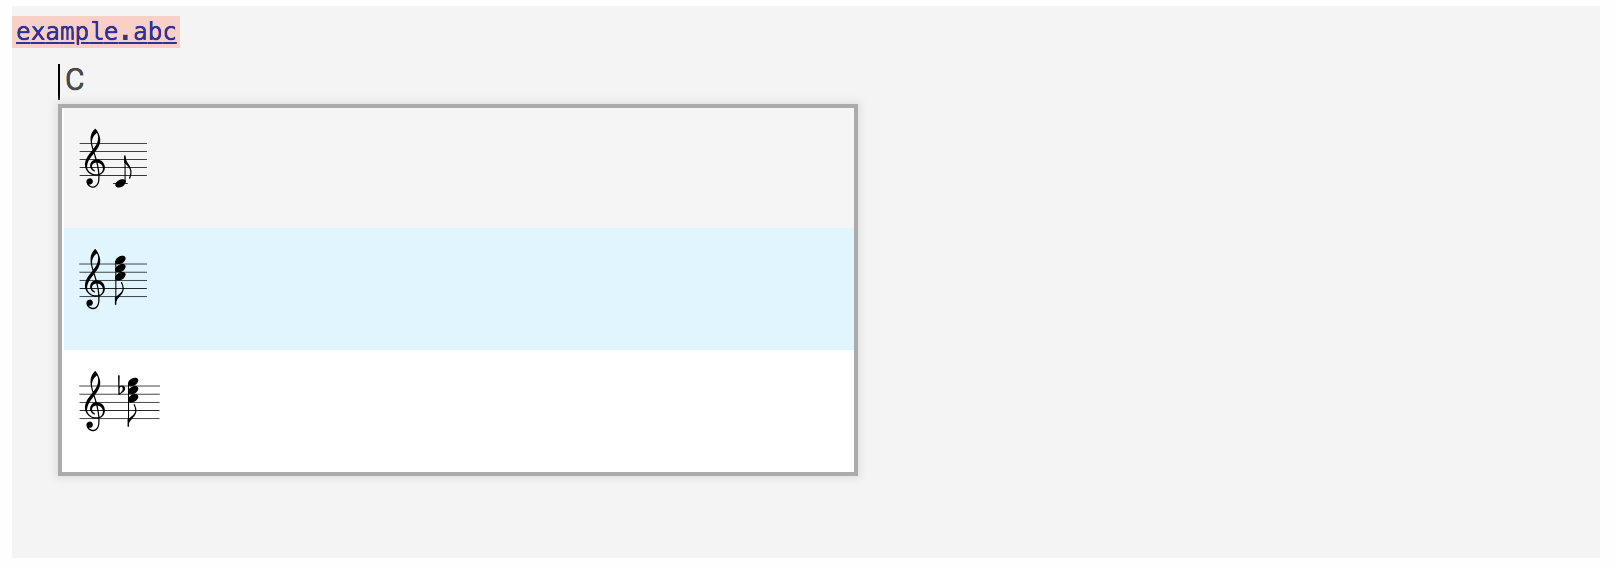
\includegraphics[width=13cm]{images/selectcandidate.png}
    \caption{変換候補選択中の画面}
    \label{select}
\end{figure}

\begin{figure}[H]
    \centering
    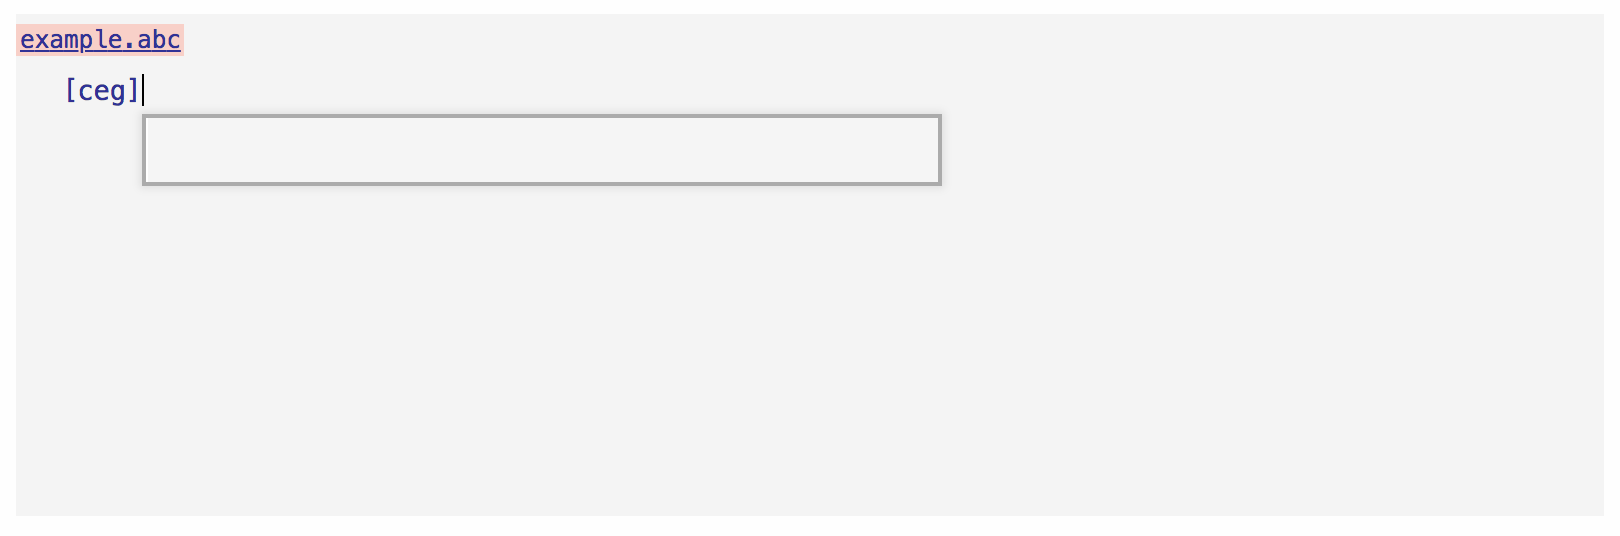
\includegraphics[width=13cm]{images/inputcandidate.png}
    \caption{変換が完了した画面}
    \label{input}
\end{figure}

\section{実装}
楽譜IMEはJavaScriptを用いてハイパー楽譜システムの内部に実装されており、ブラウザ上で利用可能である。本節では楽譜IMEのアプリケーション構成を解説する。

\subsection{文字入力}
楽譜IMEはOSから利用できるIMEとは異なり、アプリケーション自身がブラウザからキーイベントを取得する。
具体的には、ブラウザが発行するキー入力イベントがScrapboxに渡される前に横取りする形で受け取り、各種変換処理を実行している。
楽譜IME上で変換処理が確定されると、テキストエリア上の文章を操作する\texttt{Document.execCommand()}関数\footnote{\textsf{https://developer.mozilla.org/ja/docs/Web/API/Document/execCommand}}を利用してブラウザに文字入力を指示する。

\subsection{楽譜の表示}
楽譜IME起動時は楽譜プレビュー・変換候補表示用のDiv要素をScrapboxの画面上に重畳表示し、ハイパー楽譜システム同様abcjsを用いて楽譜を描画している。

\subsection{楽譜辞書}
辞書データはソースコード\ref{dict}のようなJSON形式で保持している。
辞書エントリの第1要素は楽譜の読み、第2要素は変換されるABCテキストを示している。
このような構造は既存の日本語入力システム\cite{Masui}と同様のものである。
\begin{lstlisting}[caption=楽譜IMEの辞書データ, label=dict]
[
    ["C", "[ceg]"],
    ["Cm", "[c_eg]"],
    …
]
\end{lstlisting}


\section{議論}
本節では楽譜IMEの利用において気付いた点などを述べる。
\subsection{使用感}
楽譜IMEは既存のIMEと同様のインターフェースを提供しており、入力の対象が楽譜となっても候補が表示されたり候補を選択したりする感覚は共通であることから、快適に楽譜を入力できた。
一方で、楽譜辞書のエントリ数が少ないため、思うような変換ができない場面もあった。

\subsection{辞書の編集}
現在、楽譜IMEの辞書は筆者自身が編集している。
和音を中心にエントリを追加しているが、幅広いシーンで変換機能を利用するためには辞書の充実が求められる。
しかし、コードネームやスケールといった一般的な音楽知識でさえジャンルや文脈によって名前が異なることがあり、開発者1人で網羅的な辞書を作成するのは大変困難な作業である。
単語と楽譜が対応するような辞書は存在しないので、Lexierra\cite{Masui}のようにWiki上で辞書を編集する手法が有効であると考えられる。
Wikiを利用することでソーシャルに辞書を編集できるため、膨大なエントリを協力して編集したり、ユーザーそれぞれが必要なエントリを自由に追加するといったことが可能になる。
またScrapbox上で辞書を構築すればハイパー楽譜システム・楽譜IMEを利用できるため、効率的な楽譜辞書編集が可能となる。

\subsection{動的な辞書}
ページ内外の別の楽譜をそのまま利用したいシーンがあった。
コピー\verb|&|ペーストでも対応できるが、事前に用意した楽譜辞書だけでなく、Scrapboxプロジェクト内の楽譜から動的に辞書を構築できれば、より柔軟な楽譜入力が実現できると考えられる。
また前述のソーシャルな辞書編集環境が実現された場合、ユーザーそれぞれが必要なエントリを自由に追加できるが、あるユーザーにとっては不要なエントリが変換候補として提案されてしまう可能性がある。
用途に合わせて利用する辞書を切り替えたり、エントリを絞り込むことができれば解決できると考えられる。

\section{まとめ}
ハイパー楽譜システム上で利用可能な楽譜IMEを提案した。
日本語入力システムの仕組みをABCに適用し、楽譜辞書によってABC入力を支援するシステムを実現した。
Wikiによるソーシャルな辞書編集環境や動的な辞書を実装し、あらゆる楽譜入力シーンで利用できるIMEとして拡張を行っていく予定である。